\chapter{离子推进}

\section{概述}

  现有电推进的主流方案，得到较多的应用，特点是：\textbf{高比冲}（特征值3000S），\textbf{推力小}（特征值100mN量级），\textbf{寿命长}（上万小时），\textbf{结构与配电系统复杂}
  
  主要的类型有：电子轰击式、微波电子回旋共振式、射频式。

\section{工作原理}
  一个典型的离子推进器主要由以下几个部分组成：\textbf{放电室、光学系统（栅极）、中和器}。

  \textbf{电子轰击式：}在离子源内部有空心阴极发射电子，电子轰击中性气体原子，使其电离。随后放电室内光学系统抽取等离子体中的离子并加速喷出产生推力。

  \textbf{微波电子回旋共振式：}采用处于磁场中的微波产生等离子体，无需空心阴极无需在放电室中保持直流放电。
  
  微波在输入的频率与电子回旋频率相等时铜鼓共振加速电子，从而高速电子与中性原子碰撞电离。电子回旋频率：$ \omega_c = \frac{eB}{m_e} $ 通过\textbf{调整磁场}使得在放电室的某一位置上微波电场的极化频率 $\omega$ 与电子回旋频率相等。一般的有微波频率为2.45GHz，磁场强度为875G。

  \textbf{射频离子推力器：}基本结构中放电室为\textbf{石英或氧化铝}材质，缠绕射频发生感应线圈。

  射频线圈在放电室内刑场感应电场，感应电场通过电感耦合加速电子，电子轰击中性原子产生等离子体，同样不需要空心阴极。其中电感耦合放电通过线圈上的射频电流在放电室内形成射频狡辩磁场，进而产生交变电场，装置内无电极无需外加磁场.

  \begin{table}[htbp]
    \centering
    \caption{三种离子推力器对比}
    \begin{tabular}{lcccl}
      \toprule
      & 放电阴极 & 磁场 & 电源数量 & 效率 \\
      \midrule
      电子轰击式 & 需要 & 需要 & 多 & 高，效率随尺寸的增大而增大 \\
      射频式     & 不需要 & 不需要 & 较少 & 稍低，效率随尺寸的增大而增大 \\
      微波ECR式  & 不需要 & 需要 & 较少 & 稍低，效率不随尺寸的增大而增大 \\
      \bottomrule
    \end{tabular}
  \end{table}

\section{性能参数}
  \subsection{推力}
    加速电压与离子速度的关系可以表示为：其中V为加速电压（屏栅电压或束流电压$V_b$），$v_i$为离子速度，M为离子质量，q为离子电荷
    \begin{equation}
      q V = \frac{1}{2} M v_i^2
    \end{equation}

    \textbf{理论推力}计算：其中$\eta_m$为推进剂利用效率
    \begin{equation}
      T = \dot{m}_p v_ex \approx \dot{m}_o v_i = \dot{m}_p \eta_m v_i
    \end{equation}  

    因此：
    \begin{equation}
      \left.\begin{aligned}
        \eta_m = \frac{\dot{m}_i}{\dot{m}_p} = \frac{I_b M}{e} \frac{1}{\dot{m}_p} & \\
        v_i = \sqrt{\frac{2V_b e }{M}} &
      \end{aligned} \quad \right\} \Rightarrow T = \sqrt{\frac{2M}{e}} I_b \sqrt{V_b}
    \end{equation}

    纳入损失项$\gamma = F_t \alpha$，其中$F_t$为束流发散引起的余弦损失，$\alpha$为放电室中的双电荷离子对于推力的影响：
    \begin{equation}
      T = \gamma \sqrt{\frac{2M}{e}} I_b \sqrt{V_b}
    \end{equation}

    特别的，对氙气有：
    \begin{equation}
      T = (\gamma) 1.65 I_b \sqrt{V_b} \quad [mN] \quad \quad I_b[A], V_b[V]
    \end{equation}
  
  \subsection{比冲}
    比冲的计算公式：
    \begin{equation}
      I_{sp} = \frac{T}{\dot{m}_p g_0} = \frac{\dot{m}_p \eta_m v_i}{\dot{m}_p g_0} = \frac{\eta_m v_i}{g_0} = \frac{\eta_m \sqrt{2V_b e / M}}{g_0}
    \end{equation}

    引入损失项则有：
    \begin{equation}
      I_{sp} = \frac{\gamma \eta_m \sqrt{2V_b e / M}}{g_0}
    \end{equation}

  \subsection{效率}
    \textbf{电效率}：束流功率与推力器输入功率之比
    \begin{equation}
      \eta_e = \frac{P_b}{P_{in}} = \frac{I_b V-b}{P_{in}} = \frac{I_b V_b}{I_b V_b + P_0}
    \end{equation}

    \textbf{推力效率}：喷气功率与输入功率之比
    \begin{gather}
      P_{jet} = \frac{T^2}{2\dot{m}_p} \\
      T = \dot{m}_p \eta_m v_i =\gamma \sqrt{\frac{2M}{e}} I_b \sqrt{V_b}\\
      \eta_t = \frac{P_{jet}}{P_{in}} = \gamma^2 \eta_m \frac{I_b V_B}{P_{in}}
    \end{gather}

    因此二者关系为：
    \begin{equation}
      \eta_t = \gamma^2 \eta_m \eta_e
    \end{equation}

    \textbf{要提高推进效率需要提高放电效率或推进剂利用率}
  
\section{发展历史}
  \textit{算了吧lol。}

\section{放电室}
  \subsection{结构设计与供电：}
    结构为圆柱形或圆柱形加锥段。加入锥段作用为：提高放电室结构稳定性、近小放电室离子的损失面积。\textbf{放电室功能}：为等离子体提供容器、在电离过程中充当阳极、作为整个推力器的支撑结构。

    \begin{figure}[htbp]
      \centering
      \begin{minipage}[t]{0.45\textwidth}
        \centering
        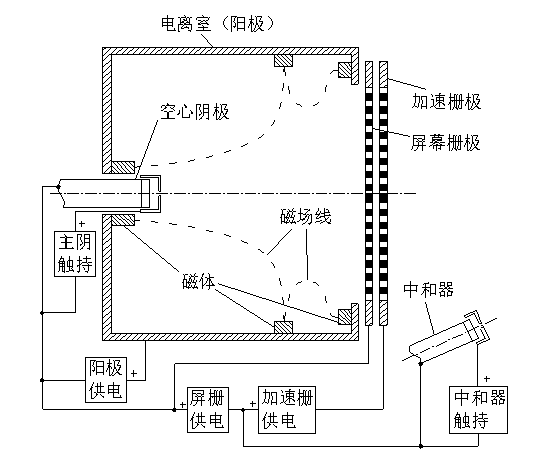
\includegraphics[width=\textwidth]{imgs/IonThruster_供电1.png}
        \caption{离子推力器供电原理图（一）}
        \label{fig:ion_thruster_power1}
      \end{minipage}
      \hfill
      \begin{minipage}[t]{0.45\textwidth}
        \centering
        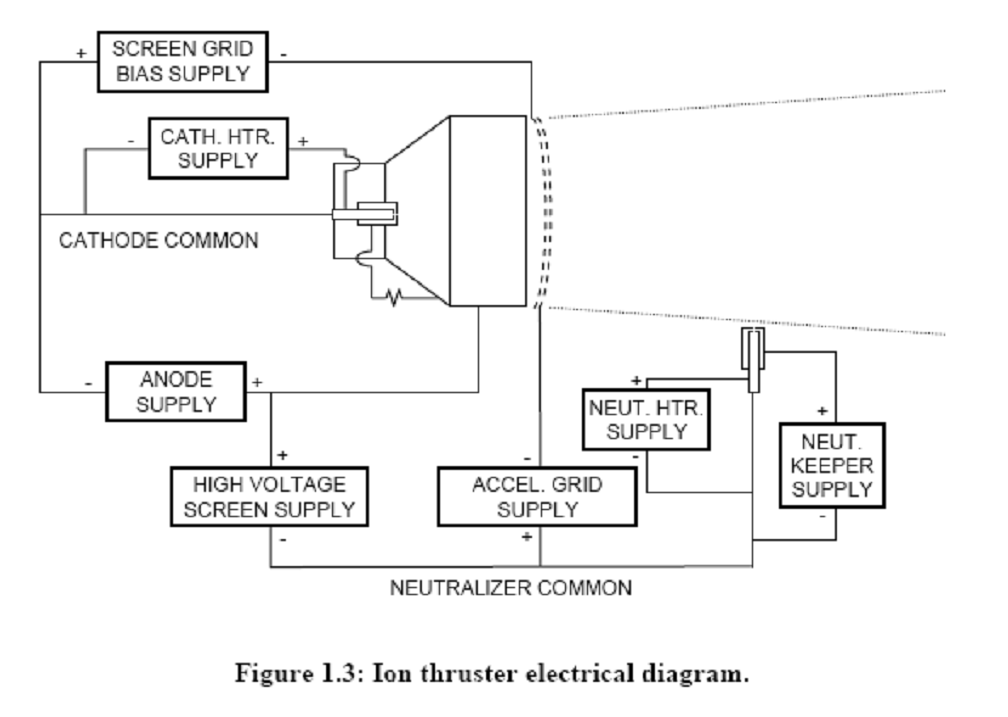
\includegraphics[width=\textwidth]{imgs/IonThruster_供电2.png}
        \caption{离子推力器供电原理图（二）}
        \label{fig:ion_thruster_power2}
      \end{minipage}
      \caption{离子推力器供电原理示意图}
      \label{fig:ion_thruster_power}
    \end{figure}

    \begin{enumerate}
      \item 阳极电位比阴极电位高20-40V
      \item 阴极电位与屏栅极电位相等
      \item 屏栅极电位约1000V，决定引出离子的能量
      \item 加速栅电位-200V，阻止下游电子反流
    \end{enumerate}

    \textbf{连接方式差异：}方式2相比方式1，高压侧电源直接升高的阳极的1040V，随后再降低到1000V提供给阴极和屏蔽栅。

    \begin{enumerate}
      \item 阳极：1个
      \item 空心阴极：3个（阴极电源，加热电源，触持电源）
      \item 屏栅：1个
      \item 加速栅：1个
      \item 中和器：3个（阴极电源，加热电源，触持电源）
    \end{enumerate}

  \subsection{磁场：}
    核心作用是：\textbf{1、约束放电室中的等离子体，提高放电效率}，没有磁场的推力器放电室是几乎无法工作的\textit{（毕竟刚电离出来就必然会撞击壁面损失掉）}。\textbf{2、约束空心阴极发射的初始电子}，原初电子的密度极低，运动自由程远大于放电室尺寸，不加限制会导致大部分原初电子撞击阳极损失。

    现实中的磁场构型：发散场、径向场、多极场、尖角场、环尖场。然而实际应用的主要仅有：发散螺线管磁场和\textbf{环尖磁场}。

    \textbf{环形会切磁场：}通过多个磁铁组成唤醒的会切磁场，磁力线种植于阳极表面，一般使用钐钴永磁体（SmCo）。优势：重量更低，束流均匀度更高，放电电压更高

    \textbf{柱形会切磁场：}优势——放电损耗低，缺点——质量相对更大（由于要加入磁靴组件）。

  \subsection{放电室性能参数：}
    \textbf{推进剂利用效率：}使用$I_n = \dot{m}_p e$表示放电室中性原子的流量（以电流形式表示），$I_b$表示从栅极引出的离子束电流
    \begin{equation}
      \eta_m = \frac{\dot{m}_i}{\dot{m}_p}
    \end{equation}

    \textbf{束流离子生成耗费}（放电损耗）：产生单位束流的等离子体消耗的额外能量：
    \begin{equation}
      \epsilon_b = \frac{(I_d - I_v) V_d}{I_b} \approx \frac{I_d V_d}{I_b}
    \end{equation}
    与电效率的关系为：
    \begin{equation}
      \eta_e = \frac{I_b V_b}{I_d V_d} = \frac{V_b}{V_d + \epsilon_b}
    \end{equation}

    \textbf{束流均匀度：}由临界磁力线和栅极组成的初始电子区形状发射束流轮廓近似互为镜像$j_{i,avg}$表示束流密度平均值；$j_{i,peak}$表示束流密度峰值
    \begin{equation}
      f_P = \frac{j_{i,avg}}{j_{i,peak}}
    \end{equation}
    \begin{figure}[htbp]
      \centering
      \begin{minipage}[t]{0.32\textwidth}
        \centering
        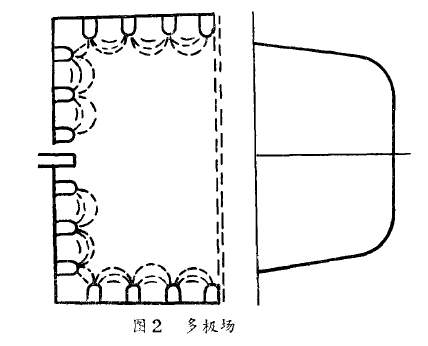
\includegraphics[width=\textwidth]{imgs/束流1.png}
        \label{fig:beam_profile1}
      \end{minipage}
      \hfill
      \begin{minipage}[t]{0.32\textwidth}
        \centering
        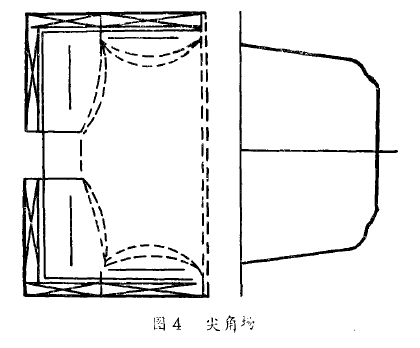
\includegraphics[width=\textwidth]{imgs/束流2.png}
        \label{fig:beam_profile2}
      \end{minipage}
      \hfill
      \begin{minipage}[t]{0.32\textwidth}
        \centering
        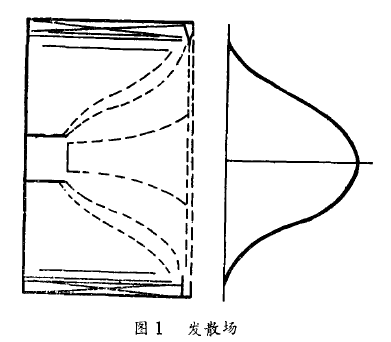
\includegraphics[width=\textwidth]{imgs/束流3.png}
        \label{fig:beam_profile3}
      \end{minipage}
      \caption{束流均匀度示意图}
      \label{fig:beam_profiles}
    \end{figure}

  \subsection{等离子体与放电电流}

  \begin{table}[htbp]
    \centering
    \caption{放电室等离子体组成}
    \renewcommand{\arraystretch}{1.2}
    \begin{tabular}{lp{0.65\textwidth}}
      \toprule
      组分 & 描述 \\
      \midrule
      原初电子 & 沿着阴极附近的发散磁场运动，并在放电室内部被磁场不断反射，最后碰撞损失能量或通过磁尖抵达阳极 \\
      二次电子 & 中性原子被轰击电离后产生的电子 \\
      离子     & 电离产生的离子（一价、二价），部分撞击壁面损失，部分由光学系统被引出产生推力 \\
      中性原子 & 未电离的原子，不受磁场约束，若不被电离则直接从栅格孔中流出 \\
      \bottomrule
    \end{tabular}
  \end{table}


  \begin{table}[htbp]
    \centering
    \caption{放电室电流组成}
    \begin{tabular}{cll}
      \toprule
      位置 & 符号 & 含义 \\
      \midrule
      \multirow{2}{*}{阴极} & $I_e$ & 阴极电子电流 \\
                            & $I_k$ & 返回到阴极的离子电流 \\
      \midrule
      \multirow{3}{*}{阳极} & $I_L$  & 阳极原初电子电流 \\
                            & $I_a$  & 阳极二次电子电流 \\
                            & $I_{ia}$ & 阳极离子电流 \\
      \midrule
      \multirow{2}{*}{栅极} & $I_B$ & 离子束流电流（栅极引出） \\
                            & $I_s$ & 屏栅极电流（撞击屏栅） \\
      \bottomrule
    \end{tabular}
  \end{table}

  放电室电流平衡有：
  \begin{gather}
    I_e = I_d - I_s -I_k\\
    I_a = I_d + I_{ia} - I_L
  \end{gather}

  \textbf{放电电流测量：}实验方法、零维模型方法，PIC-MCC方法。

  \textbf{放电室等离子体分布：}（典型情况）
  \begin{figure} [htbp]
    \centering
    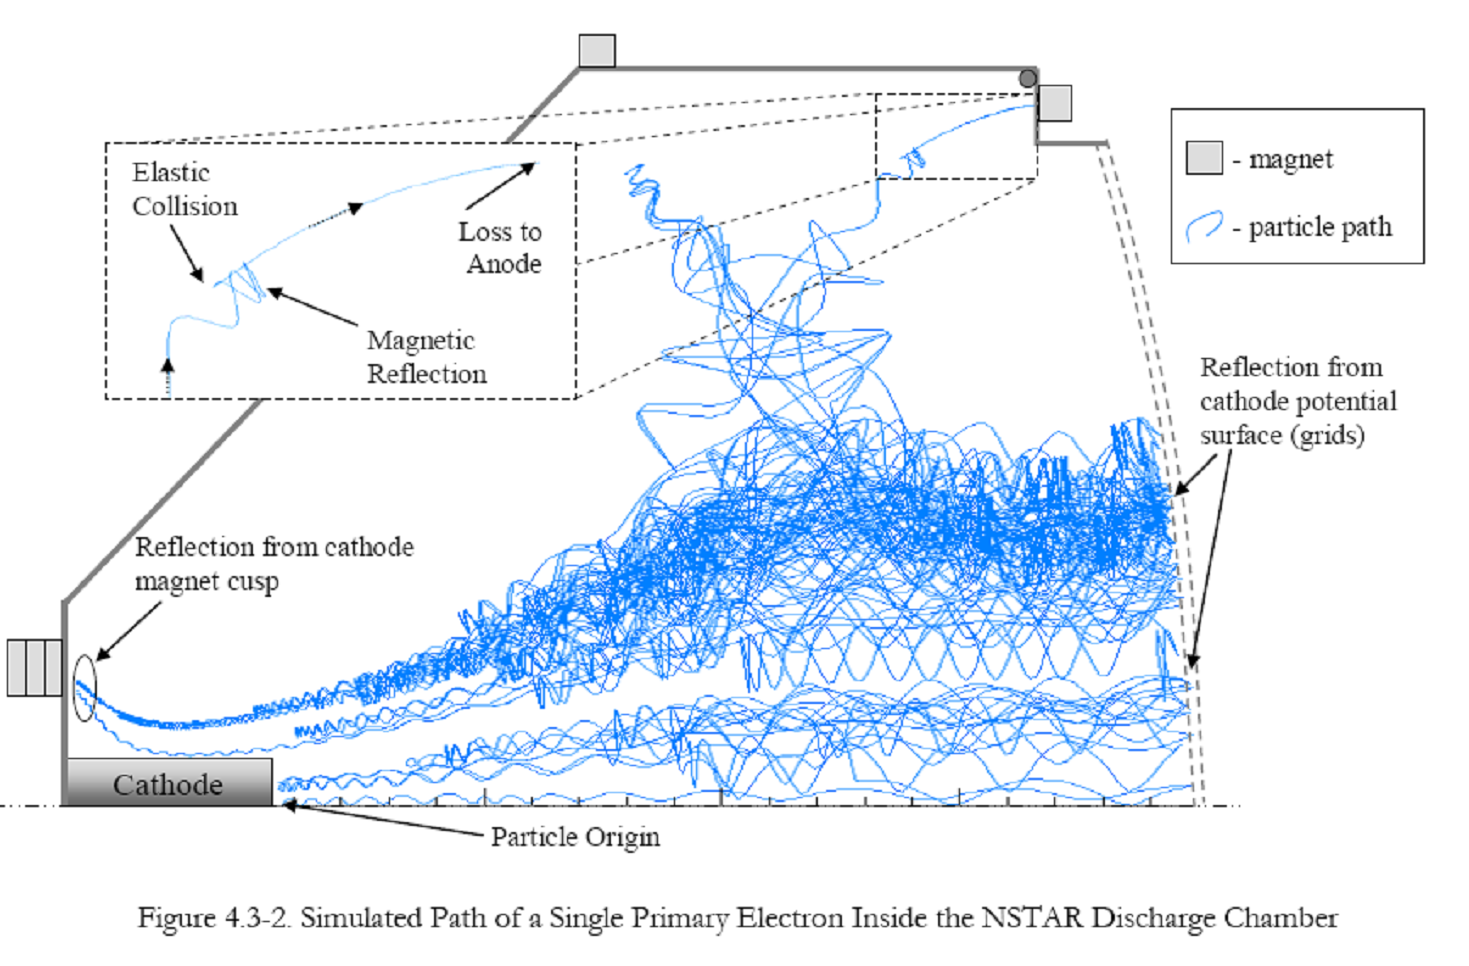
\includegraphics[width=0.7\textwidth]{imgs/原初电子分布.png}
    \caption{放电室原初电子分布示意图}
    \label{fig:primary_electron_distribution}
  \end{figure}

\section{栅极组件}

  \subsection{栅极组成与功能}
  双栅极系统：屏蔽栅（1000V）+加速栅（-200V），屏蔽栅用于引出离子束流，加速栅用于阻止下游电子反流。\textbf{屏蔽栅作用}：将放电室等离子体的边界限制在栅极上游、将等离子体中的电子限制在放电室内（屏栅电压低于阳极）、将离子聚焦引出\textbf{加速栅作用}：进一步增加离子束流的引出，并阻止下游电子反流。

  三栅极系统：屏蔽栅（1000V）+加速栅（-200V）+减速栅（0V），\textbf{减速栅作用}：电势趋近于0，有效减小下游电荷交换对于栅极的溅射腐蚀。

  \textbf{加工与装配：}屏栅与加速栅的极孔必须按照设计实现\textbf{对中}。一般蚕蛹钼、钛、CC复合材料，采用液压成型的方式制造。其中CC复合材料具有负的热膨胀系数，可以加工为平面。钼栅极需要加工为球面（或凹面）以补偿热膨胀导致的栅极短路。

  \subsection{束流引出与聚焦}

  \textbf{交叉基线与导流极限：}抽取电流过小或放电室等离子体密度过小——推力器工作在交叉极限。抽取电流过大或放电室等离子体密度过大——推力器工作在导流极限。
  \begin{figure} [htbp]
    \centering
    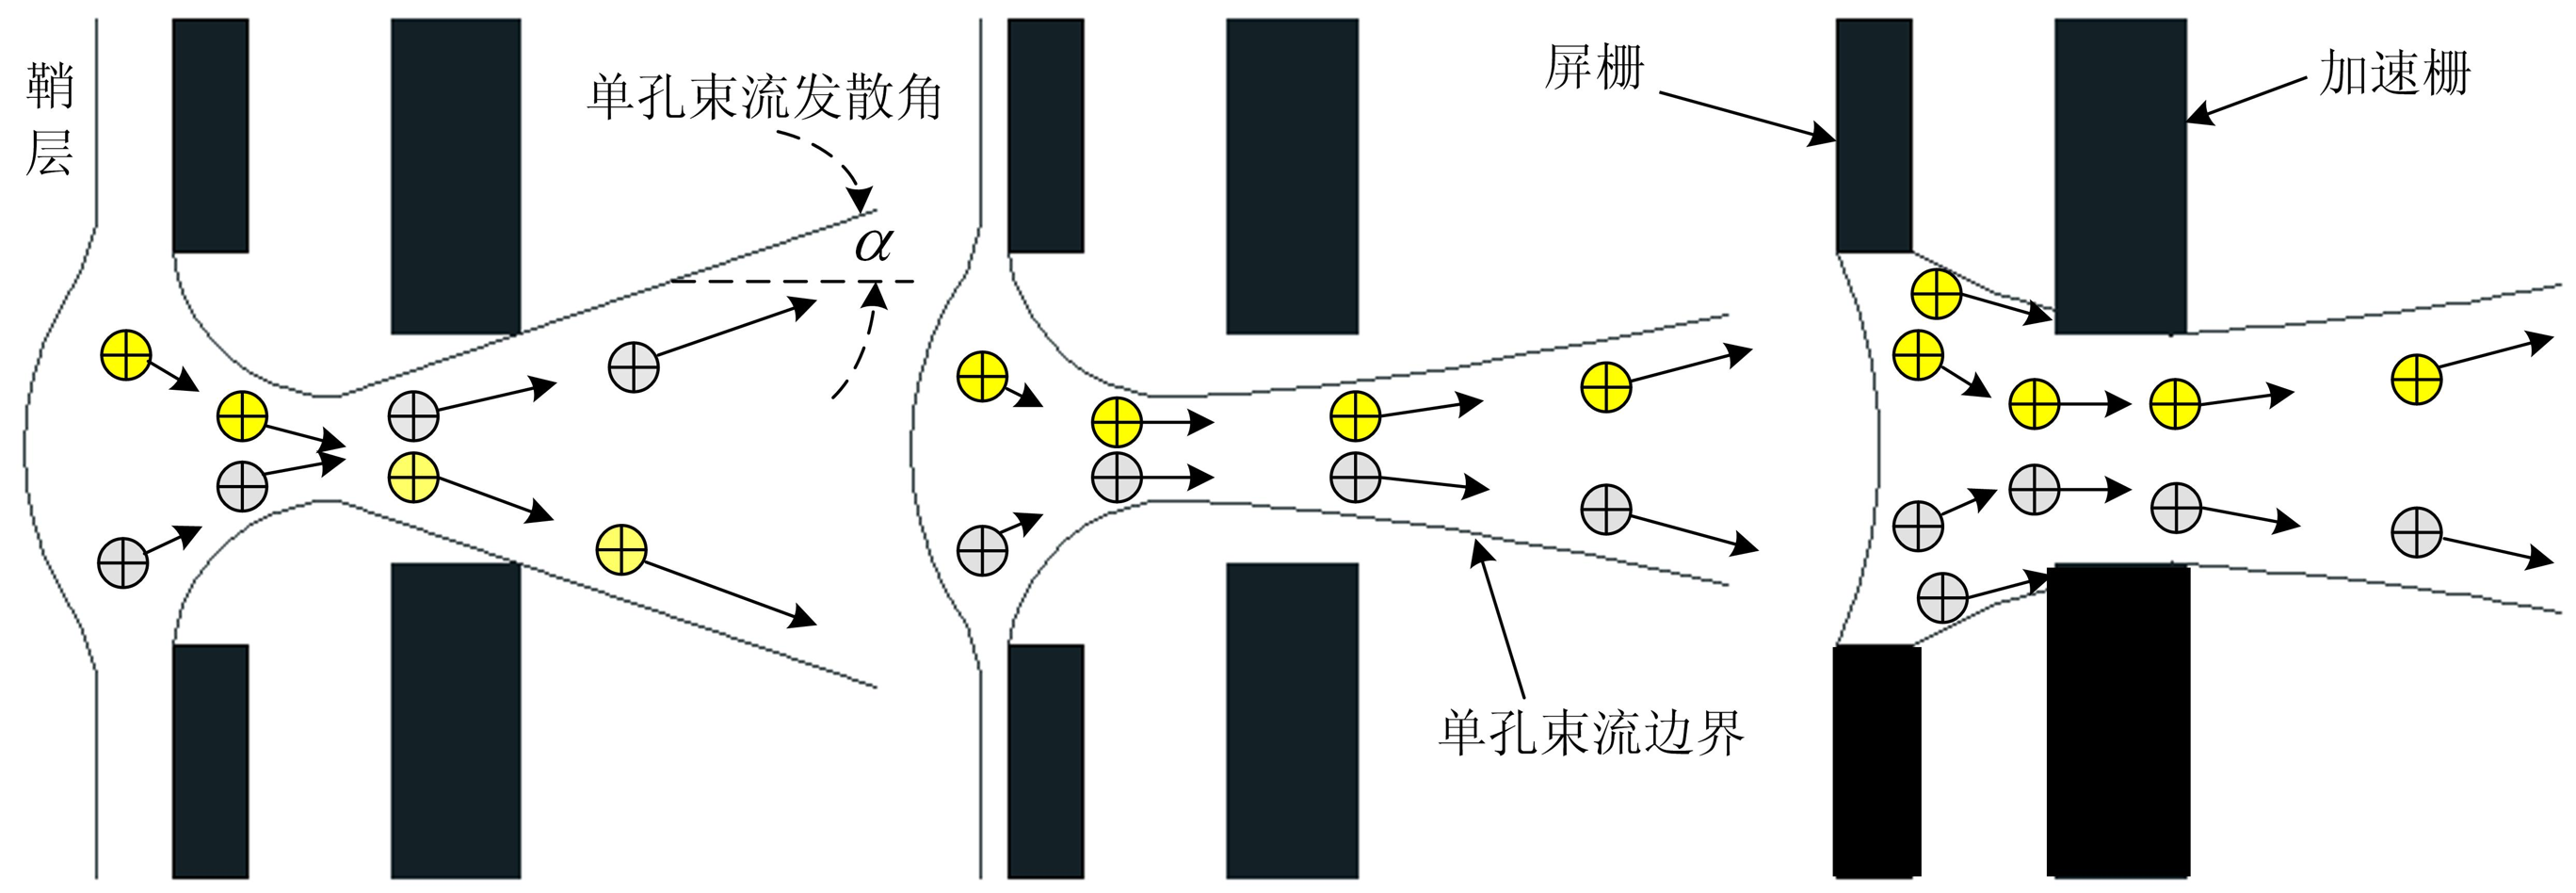
\includegraphics[width=0.5\textwidth]{imgs/束流引出状态.png}
    \caption{束流引出极限示意图}
    \label{fig:beam_extraction_limit}
    \small （左-交叉极限，中-正常聚焦，右-导流极限）
  \end{figure}

  \textbf{放电室等离子体密度影响：}等离子体密度\textbf{越大}，上游鞘层约靠近屏栅位置，束流越接近导流极限。

  \textbf{屏栅电压影响：}在加速栅电压不变的情况下，随着屏栅电压的降低，逐渐出现欠聚焦的情况。

  \begin{figure} [htbp]
    \centering
    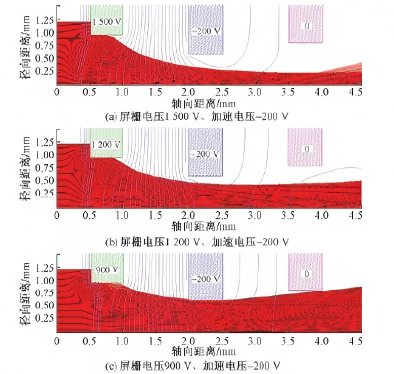
\includegraphics[width=0.5\textwidth]{imgs/屏栅电压对于束流影响.png}
    \caption{屏栅电压对于束流聚焦的影响示意图}
    \label{fig:beam_focusing_state}
  \end{figure}

  \textbf{静总加速电压比}：定义离子束中离子的静加速电压与总加速电压之比，其中$V_P$为等离子体电位，$V_S$为屏栅电位，$V_A$为加速栅电位（由于供电伏电压，需要加入绝对值）

  \begin{equation}
    R = \frac{V_N}{V_T} = \frac{V_P+V_S}{V_P+V_S+|V_A| }
  \end{equation}

  静总加速电压比反应加速场与减速场对于离子的聚焦与散焦的程度，决定推力器的\textbf{束发散角$\alpha$}，一般R越大，束流发散角越小，通常设计中取0.85$\thicksim $0.9。

  \subsection{束流密度极限（Child-Langmiur）}

  假设两个无限大的平面带点极板，其位置与电势分别为$x = 0, \varphi = 0$与$x = d, \varphi = V_0$。质量为$m$的带电粒子从x=0处以0初速发射，计算两极板间的电流密度。

  额外的边界条件为 x=0 处电场为0，即$\frac{\partial \varphi}{\partial x}(0) = 0$。需要满足的方程为：
  \begin{gather}
    \frac{\partial^2 \varphi}{\partial x^2} = -\frac{\rho(x)}{\epsilon_0} \quad \text{（泊松方程）} \\
    \frac{1}{2} m v^2 = e \varphi(x) \Rightarrow v(x) = \sqrt{\frac{2e\varphi(x)}{m}} \quad \text{（能量守恒）} \\
    j = \rho(x) v(x) \Rightarrow |\rho(x)| = \frac{j}{v(x)} = j \sqrt{\frac{m}{2e\varphi(x)}} \quad \text{（连续性方程）}
  \end{gather}

  带入泊松方程可以得到：
  \begin{equation}
    \frac{\partial^2 \varphi}{\partial x^2} = -\frac{j}{\epsilon_0} \sqrt{\frac{m}{2e\varphi(x)}}
  \end{equation}

  为了方便求解，我们先对等式右边的常数项进行合并。令常数：
  \begin{equation}
    C = -\frac{j}{\epsilon_0} \sqrt{\frac{m}{2e}}
  \end{equation}

  原方程可以简化为：
  \begin{equation}
    \frac{d^2 \varphi}{d x^2} = C \varphi^{-1/2}
  \end{equation}

  这是一个二阶非线性微分方程，标准求法是利用\textbf{降阶法（乘以一阶导数）}。以下是具体的积分求解步骤。

  \medskip
  \textbf{第一步：方程两边同乘以 $\displaystyle \frac{d\varphi}{dx}$}
  \begin{equation}
    \frac{d^2 \varphi}{d x^2} \cdot \frac{d\varphi}{dx} = C \varphi^{-1/2} \cdot \frac{d\varphi}{dx}
  \end{equation}

  注意到左边可以写成全微分的形式：
  \begin{equation}
    \frac{d^2 \varphi}{d x^2} \cdot \frac{d\varphi}{dx} = \frac{1}{2} \frac{d}{dx} \left( \frac{d\varphi}{dx} \right)^2
  \end{equation}

  代入后，方程变为：
  \begin{equation}
    \frac{1}{2} \frac{d}{dx} \left( \frac{d\varphi}{dx} \right)^2 = C \varphi^{-1/2} \frac{d\varphi}{dx}
  \end{equation}

  \medskip
  \textbf{第二步：对 $x$ 进行第一次积分}

  两边同时对 $x$ 积分（等价于右边直接对 $\varphi$ 积分）：
  \begin{gather}
    \frac{1}{2} \left( \frac{d\varphi}{dx} \right)^2 = \int C \varphi^{-1/2} d\varphi \\
    \frac{1}{2} \left( \frac{d\varphi}{dx} \right)^2 = 2C \varphi^{1/2} + C_1
  \end{gather}

  \textit{边界条件简化：在物理实际中（例如阴极表面 $x=0$ 处），通常假设电势 $\varphi(0) = 0$ 且电场强度 $-\frac{d\varphi}{dx} \big|_{x=0} = 0$。如果是这种情况，积分常数 $C_1 = 0$。为了推导简洁，我们假设 $C_1 = 0$ 继续求解（若 $C_1 \neq 0$，则需要用到椭圆积分，形式会极其复杂）。}

  在 $C_1 = 0$ 的情况下：
  \begin{gather}
    \left( \frac{d\varphi}{dx} \right)^2 = 4C \varphi^{1/2} \\
    \frac{d\varphi}{dx} = 2\sqrt{C} \varphi^{1/4} \quad \text{（取正根，假设电势随距离增加）}
  \end{gather}

  \medskip
  \textbf{第三步：分离变量进行第二次积分}

  将关于 $\varphi$ 和 $x$ 的项分离开来：
  \begin{equation}
    \varphi^{-1/4} d\varphi = 2\sqrt{C} dx
  \end{equation}

  两边同时积分：
  \begin{gather}
    \int \varphi^{-1/4} d\varphi = \int 2\sqrt{C} dx \\
    \frac{4}{3} \varphi^{3/4} = 2\sqrt{C} x + C_2
  \end{gather}

  再次利用边界条件，若 $x=0$ 时 $\varphi=0$，则 $C_2 = 0$：
  \begin{equation}
    \frac{4}{3} \varphi^{3/4} = 2\sqrt{C} x \;\Longrightarrow\; \varphi^{3/4} = \frac{3}{2}\sqrt{C} x
  \end{equation}

  \medskip
  \textbf{第四步：解出 $\varphi(x)$}

  两边同时 $4/3$ 次方：
  \begin{equation}
    \varphi(x) = \left( \frac{3}{2}\sqrt{C} x \right)^{4/3} = \left(\frac{9}{4} C x^2 \right)^{2/3}
  \end{equation}

  \medskip
  \textbf{最终结果（代入物理常数）}

  将最开始设定的常数 $C = -\frac{j}{\epsilon_0} \sqrt{\frac{m}{2e}}$ 代回（注意：物理上电流密度 $j$ 的方向通常会带来负号，使其整体开根号内为正，这里我们关注大小关系）：
  \begin{equation}
    \varphi(x) = \left( \frac{9j}{4\epsilon_0} \sqrt{\frac{m}{2e}} \right)^{2/3} x^{4/3}
  \end{equation}

  这就是该方程在特定边界条件下的通解。它表明，在空间电荷限制下，\textbf{电势 $\varphi$ 与距离 $x$ 的 $4/3$ 次方成正比}。

  相应的，电流密度的极限（Child-Langmuir 极限）可以通过在 $x=d$ 处代入 $\varphi(d) = V_0$ 来求得：
  \begin{equation}
    j_{max} = \frac{4\epsilon_0}{9} \sqrt{\frac{2e}{m}} \frac{V_0^{3/2}}{d^2}
  \end{equation}

  在离子推力器的光学系统中，极板间的距离d使用$l_e = \sqrt{(l_g + t_s)^2 + \left(\frac{d_s}{2}\right)^2}$表
  示，极板间的电压$V_0$用$V_T = V_P + V_S + |V_A|$表示。

  \begin{equation}
    j_{max} = \frac{4\epsilon_0}{9} \sqrt{\frac{2e}{M}} \frac{V_T^{3/2}}{l_e^2}
  \end{equation}

  \begin{figure}[htbp]
    \centering
    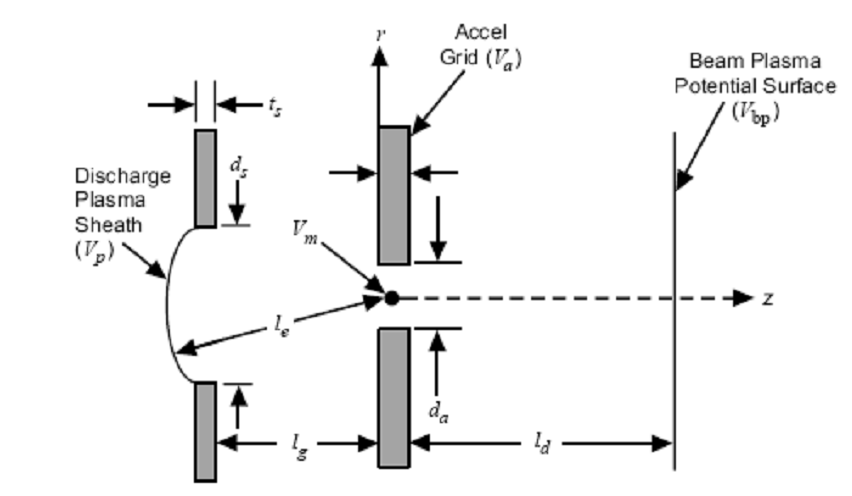
\includegraphics[width=0.45\textwidth]{imgs/栅孔尺寸系数.png}
    \caption{束流密度极限示意图}
    \label{fig:beam_density_limit}
  \end{figure}

  \textbf{因此相同推力大小下离子推力器的口径往往大于霍尔推力器，离子推力器的推力密度也明显更小}

  \textbf{归一化导流系数}：定义最大归一化导流系数为：设计时实用K值一般取$K_{max}\times 50\%$
  \begin{equation}
    K_{max} = \frac{4\epsilon_0}{9} \sqrt{\frac{2e}{M}} \quad \Rightarrow \quad K_{max,Xr} = 4.75 \times 10^{-9} \ \ [A/V^{3/2}]
  \end{equation}

  \subsection{电子回流问题}

  改变加速栅电压与加速栅孔径均会影响下游电子回流。更高的加速栅电压或更大的加速栅孔径会导致更多的电子回流。同时\textbf{放电腐蚀导致的加速栅孔径变大会导致电子回流}

  \begin{figure}[htbp]
    \centering
    \begin{minipage}[t]{0.48\textwidth}
      \centering
      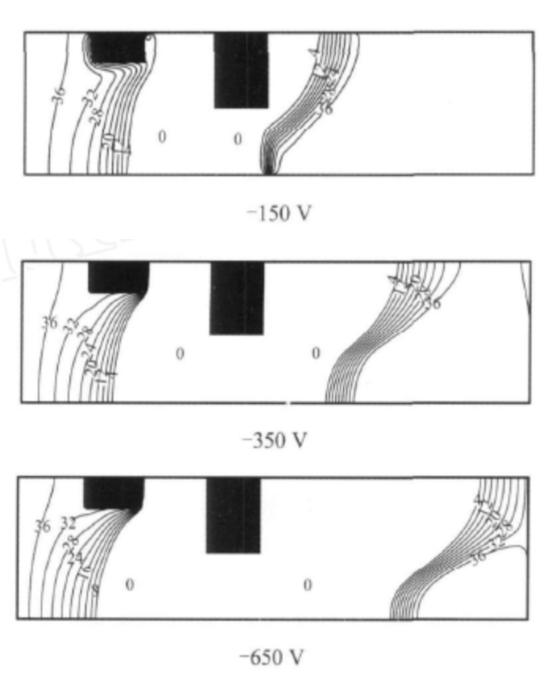
\includegraphics[height=6.5cm]{imgs/电子回流-改变加速栅电压.png}
      \caption{改变加速栅电压}
      \label{fig:electron_backstreaming_voltage}
    \end{minipage}
    \hfill
    \begin{minipage}[t]{0.48\textwidth}
      \centering
      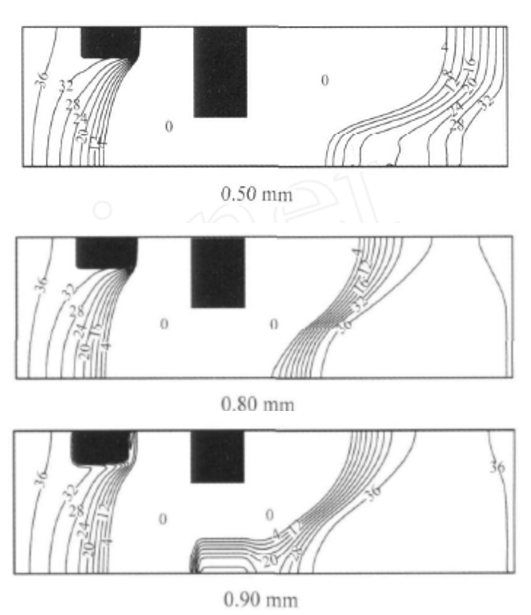
\includegraphics[height=6.5cm]{imgs/电子回流-改变加速栅孔半径.png}
      \caption{改变加速栅孔半径}
      \label{fig:electron_backstreaming_radius}
    \end{minipage}
    \caption{电子回流影响因素示意图}
    \label{fig:electron_backstreaming}
  \end{figure}

  \subsection{下游栅极腐蚀}

  在推力器羽流的下游会产生电荷交换碰撞，包括：
  \begin{gather}
    Xe^+ + Xe \rightarrow Xe + Xe^+ \\
    Xe^{++} + Xe \rightarrow Xe + Xe^{++}
  \end{gather}

  其中在加速栅下游发生的电荷交换碰撞会导致慢速的带正电的离子再次被加速栅吸引，从而轰击加速栅导致表面腐蚀：
  \begin{equation}
    Xe_{fast}^+ + Xe_{slow} \rightarrow Xe_{slow}^+ + Xe_{fast}
  \end{equation}

  \begin{figure}[htbp]
    \centering
    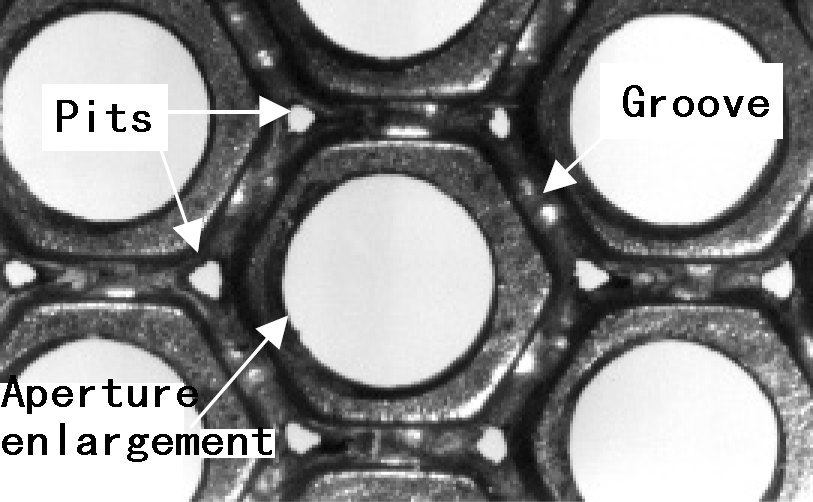
\includegraphics[width=0.3\textwidth]{imgs/栅极腐蚀效果.png}
    \caption{下游栅极腐蚀示意图}
    \label{fig:downstream_grid_erosion}
  \end{figure}

  \textbf{腐蚀率}：表示栅极表面单位时间的腐蚀深度。其中N表示单位时间射入离子个数，J表示离子射入电流密度，Y表示溅射产额——每个离子射入能够轰击出的材料原子个数，$\rho_g$被轰击的材料的密度，$M_g$表示被轰击的材料的原子质量。
  \begin{equation}
    R_E = \frac{V}{S} = \frac{ YNM_g }{ S\rho_g } = \frac{Y J M_g}{e \rho_g}
  \end{equation}

  \textbf{溅射产额}：与离子的入射能量、入射角度有关。

  \begin{figure}[htbp]
    \centering
    \begin{minipage}[t]{0.48\textwidth}
      \centering
      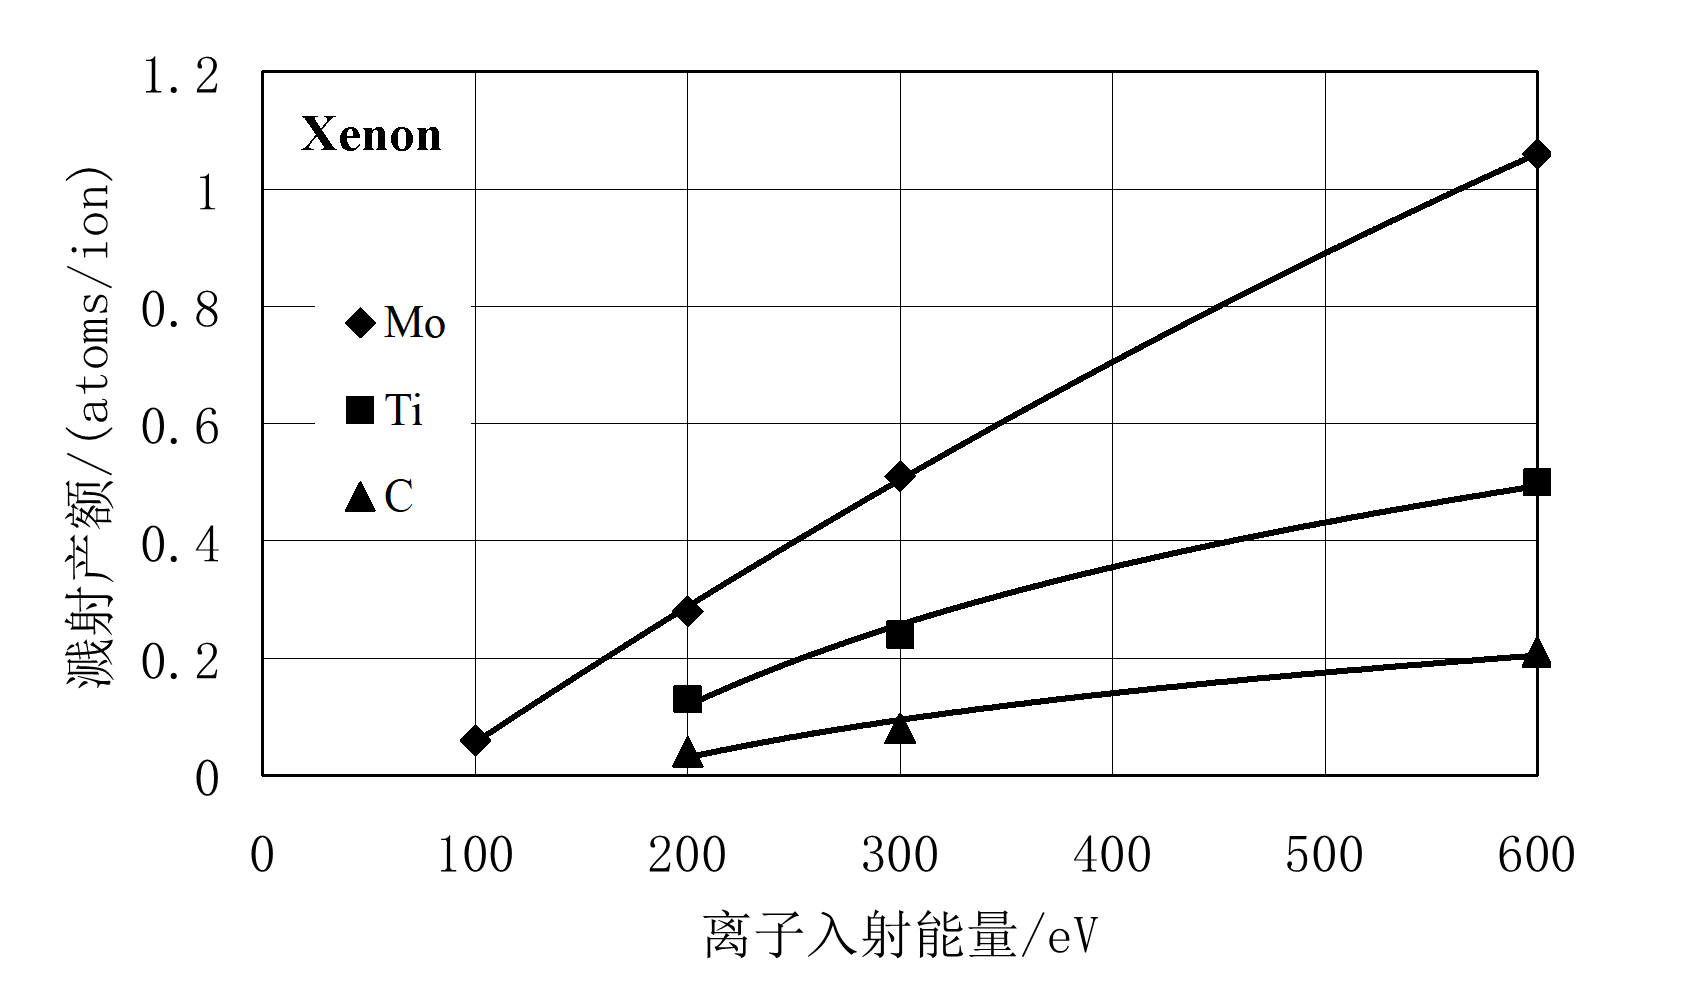
\includegraphics[height=4cm]{imgs/溅射产额-入射能量.png}
      \caption{溅射产额与入射能量的关系}
      \label{fig:sputtering_yield_energy}
    \end{minipage}
    \hfill
    \begin{minipage}[t]{0.48\textwidth}
      \centering
      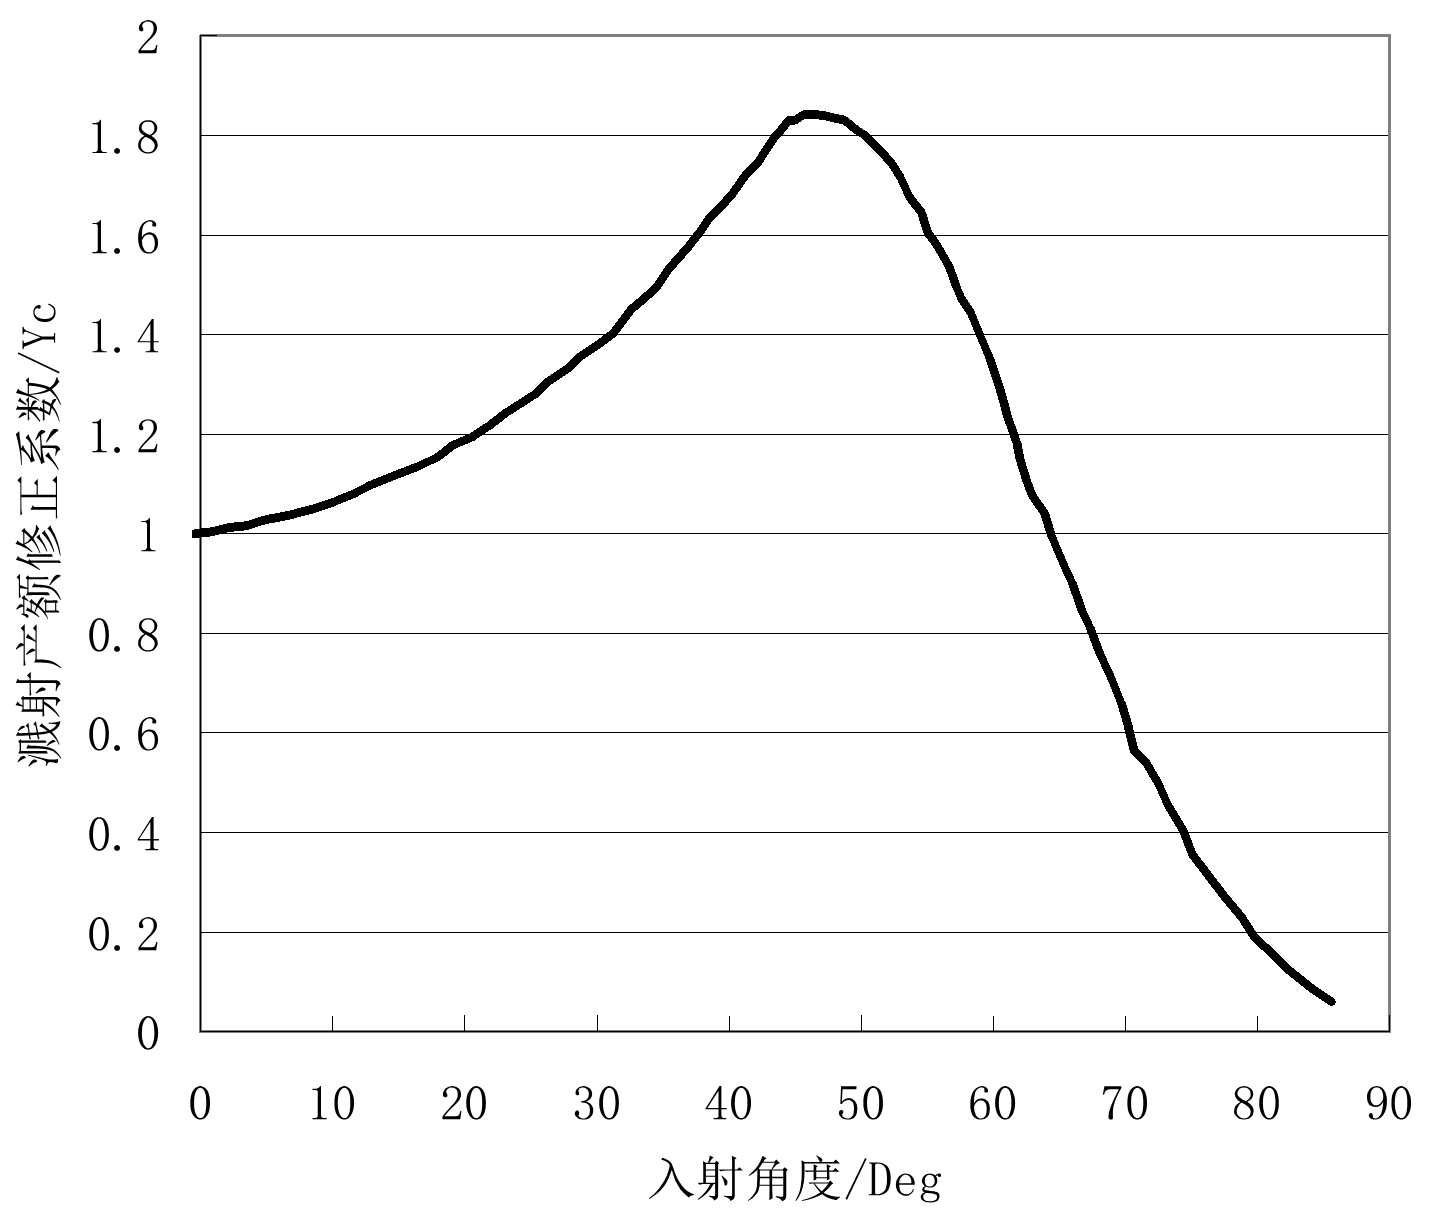
\includegraphics[height=4cm]{imgs/溅射产额-入射角度.png}
      \caption{溅射产额与入射角度的关系}
      \label{fig:sputtering_yield_angle}
    \end{minipage}
    \caption{溅射产额影响因素示意图}
    \label{fig:sputtering_yield}
  \end{figure}

  \textbf{延长寿命的措施}：采用三栅系统、降低加速栅电压、更换栅极材料。

  \subsection{栅间短路问题}
    控制栅极间距、控制放电室碎片的尺寸。

\section{推力器设计}

  \subsection{总体思路}
    \begin{enumerate}
      \item 根据任务需求与推进剂类型确定\textbf{比冲}
      \item 根据任务需要的推力与比冲确定推力器\textbf{功率}
      \item 根据推力、比冲，确定推力器所需的\textbf{束流电流}与\textbf{束流电压}
      \item \textbf{参考束流密度极限}确定束流密度并得出推力器\textbf{口径}
      \item 估算最终的\textbf{阳极电流}（为束流电流的4-7倍），并根据电流平衡关系得出主阴极\textbf{发射电流}
    \end{enumerate}
    \begin{gather}
      I_sp = \frac{\gamma \eta_m \sqrt{2V_b e / M}}{g_0} \\
      T = \gamma \sqrt{\frac{2M}{e}} I_b \sqrt{V_b} \\
      P = \frac{T I_{sp} g_0}{2 \eta_t}
    \end{gather}

    设计原则：
    
    \textbf{1、}阳极筒表面区域内形成磁场，磁力线不与阳极筒相交——实现放电等离子体的低气压化、高密度化和均匀化。
    
    \textbf{2、}理想磁力线分布是将磁场限制在阳极附近区域，使放电室内（特别是栅极附近）近似于无磁场，从而增强引出束流的分布均匀性

    \textbf{3、}锥段磁感应强度应强于柱段磁感应强度，放电室在周线上的磁场强度在阴极触持极顶部达到最大值，而柱段磁场强度要迅速衰减，从而兼顾放电效率与束流均匀性。

  \subsection{环形会切场放电室}

    主要特点：
    \begin{enumerate}
      \item 结构简单无磁靴。
      \item 除阴极与栅极外放电室为整体密封结构，无屏栅筒。
      \item 放电室受离子轰击的零件更少，只有屏栅和阴极，相应的溅射产物更少。
      \item 放电室的茨空区域较大，束流均匀性更好，更适合大口径的离子推力器。
      \item 无法使用电磁铁实现放电室的优化实验，对于磁场分布的调整只能在仿真基础上进行
    \end{enumerate}

    \textbf{放电电流设计}：考虑所要求的束流与放电损耗，一般按照如下公式进行估算：
    \begin{equation}
      I_d = (5 \sim  7) \times I_b
    \end{equation}

    \textbf{放电电压与流率设计}：考虑放电室磁场、阴极流率、推进剂利用率影响，设计原则为推进剂利用率越高越好，放电电压和放电损耗越低越好，但是三者本身存在制约关系，需要权衡考虑。一般放电电压取24-30V，放电室的工质利用率在70-95\%

    \textbf{口径设计}：通过束流密度极限确定束流口径，一般栅极的最大工作束流密度不超过其极限束流密度的60\%，放电室口径一般大于束流口径但不超过束流口径的1.2倍，放电室柱段阳极直径一般为栅极最大开孔区域直径+20至30mm。
    \begin{equation}
      J_{b,max} = K_{max,Xr} \frac{V_T^{3/2}}{l_e^2} \quad \left( K_{max,Xr} = 4.75 \times 10^{-9} \ \ [A/V^{3/2}] \right)
    \end{equation}

    \textbf{几何结构设计}：一般采用\textbf{“锥段-直段型”放电室}，既有最长的原初电子约束长度，放点效率最高，且随着口径增加优势愈发明显。

    \textbf{放电室长径比设计：}放电室较长有利于增大工质气体在推力器中的留存时间，提高工质利用率，但是较长的放电室会降低放电室中原初电子的密度，降低放电效率。一般放电室长径比在0.4到1.0之间。

    \textbf{主阴极位置}：阴极位置决定了原初电子的发射位置，阴极顶点应位于最大轴向场强处，此处的磁力线应从轴线快速向四周辐射从而使得原初电子原理中心轴，提高电离效率与束流均匀度。

    \textbf{供气方式}：束流均匀性取决于栅极上游放电室的等离子体分布的均匀性与栅极的引出性能，而其中的等离子体分布均匀性取决于原初电子分布均匀性与中性原子的浓度分布，一般采用\textbf{栅极出口反向供气}有利于提高束流均匀度。

    \textbf{磁场设计}：
    使用更多的磁极，磁间距越小，特征磁场线越接近阳极，束流均匀性越好，但是也会暴露更多磁尖带俩更多的损失面积，放电损耗更多。设计原则为：\textbf{使用最小磁极数}下，实现最佳的放电室磁场构型，同时满足磁屏蔽放电室壁，放电室大部分区域接近无场区。    磁极间距——一般取11-16cm；磁体材料——满足大磁能积、高矫顽力、高耐热性；磁体尺寸——满足放电室内闭合磁等势线为50Gauss左右，放电室出口磁场接近无场（小于5Gauss）。

    \begin{figure}[htbp]
      \centering
      \begin{minipage}[t]{0.48\textwidth}
        \centering
        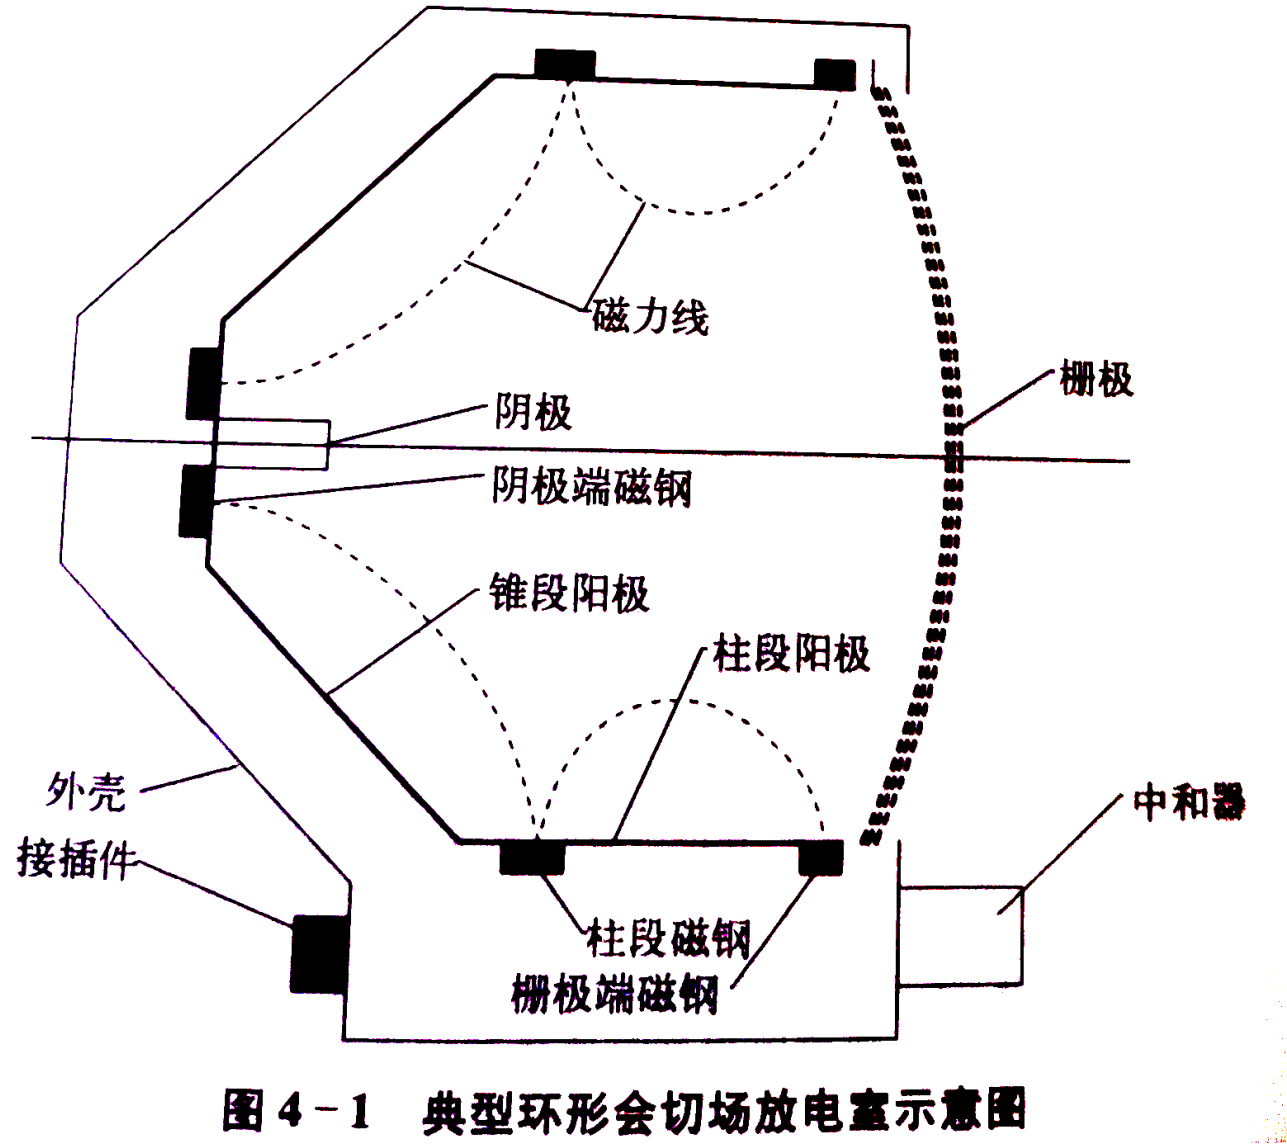
\includegraphics[height=7cm]{imgs/环形会切场结构.png}
        \caption{环形会切磁场示意图}
        \label{fig:ring_cusp_magnetic_field}
      \end{minipage}
      \hfill
      \begin{minipage}[t]{0.48\textwidth}
        \centering
        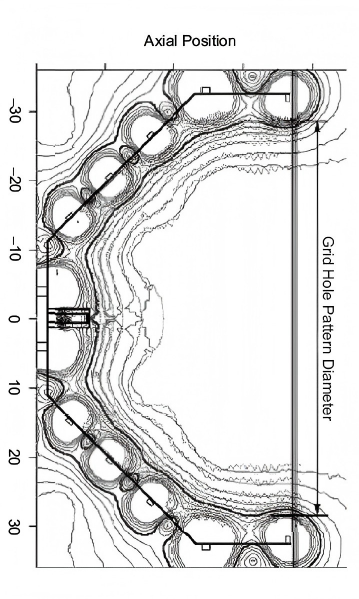
\includegraphics[height=7cm]{imgs/环形会切场磁场.png}
        \caption{环形会切磁场磁力线示意图}
        \label{fig:ring_cusp_magnetic_field_lines}
      \end{minipage}
      \caption{环形会切磁场结构示意图}
      \label{fig:ring_cusp_magnetic}
    \end{figure}

    \textbf{参数优化}：磁场优化、电气参数优化、多模式调节优化

  \subsection{柱形会切场放电室}
  
    优点：
    \begin{enumerate}
      \item 锥段磁场较强，柱段磁场较弱。
      \item 极靴深入放电室内部更有利于形成平行于阳极表面的磁场分布。
      \item 磁体位于屏蔽筒外侧降低工作温度。
    \end{enumerate}

    缺点：
    \begin{enumerate}
      \item 磁柱数量有限，周向磁场均匀性较差。
      \item 放电室需要屏蔽同于阳极筒双层结构，质量较大。
      \item 磁极深入放电室内部，有更多离子刻蚀产物的风险。
    \end{enumerate}
    
    \textbf{放电室口径：}放电室口径大于束流口径，但是不超过1.2倍数，一般取最大引出束流不超过栅极最大引出能力的60\%。有如下半经验公式：其中$I_{max}$为最大引出束流，$n$为栅孔数量，$P_{max}$为栅孔最大导流系数，$V_T$为总加速电压。
    \begin{equation}
      I_{max} \leq 0.6 \times n \times P_{max} \times V_T^{\frac{3}{2}}
    \end{equation}

    \textbf{放电室几何结构}：同样使用“锥段-直段型”放电室，既有最长的原初电子约束长度，放点效率最高，且随着口径增加优势愈发明显。

    \textbf{主阴极位置}：同样位于轴线的轴向磁场最强处，从而确保袁术电子被分散在整个放电腔当中。兼具电离效率与束流均匀度。

    \textbf{设计参数的经验公式}：
    \begin{figure}[htbp]
      \centering
      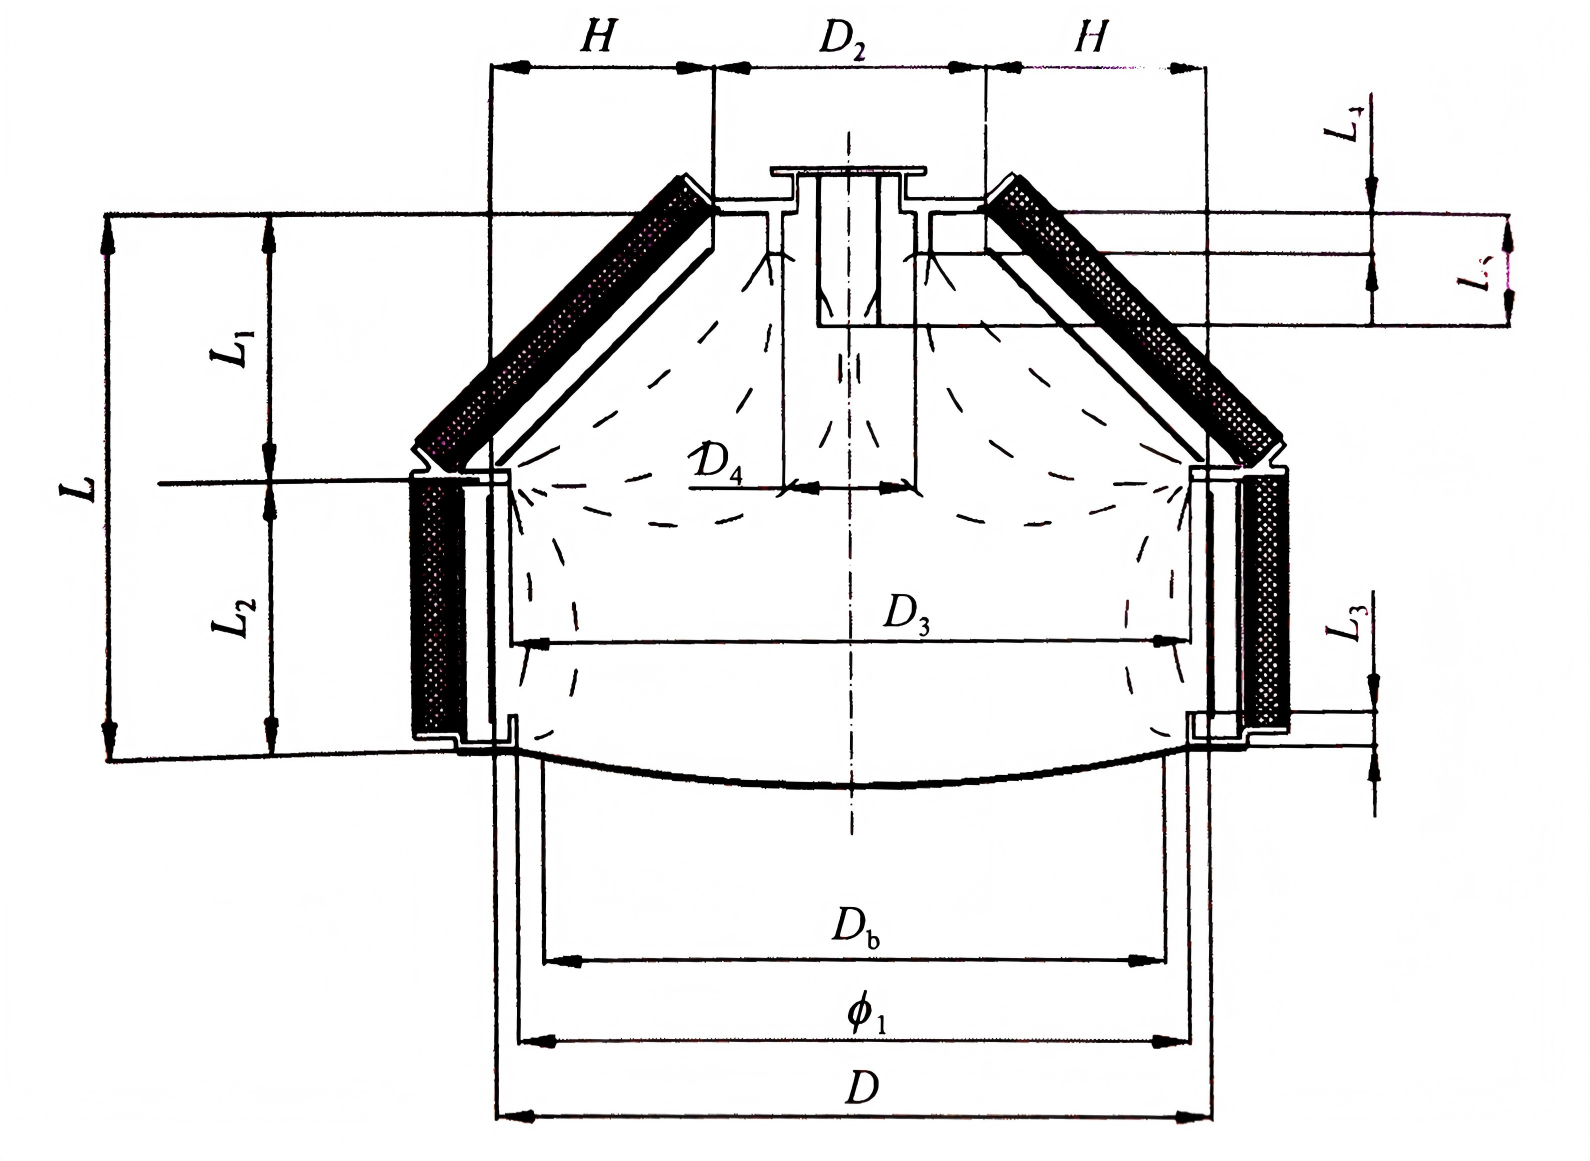
\includegraphics[width=0.7\textwidth]{imgs/柱形会切场几何参数.png}
      \caption{柱形会切磁场结构示意图}
      \label{fig:cylindrical_cusp_magnetic_field}

      \small $D_b$——束流口径\\
      $\phi_1$——上极靴内径，\:\:$\phi_2$——中极靴内径，\:\:$\phi_3$——下极靴内径\\
      $D_d$——柱段阳极筒内径，\:\:$H$——锥段阳极筒高度，\:\:$D_2$——锥段阳极筒小圆内径\\
      $L$——放电室长度，\:\:$L_1$——放电室锥段长度，\:\:$L_2$——放电室直段长度\\
      $L_3$——上极靴长度，\:\:$L_4$——下极靴长度，\:\:$L_5$——阴极深入放电室长度
    \end{figure}

    \begin{gather}
      D_d = D_h +28 \\
      L/D_d = \frac{2}{3} \\
      L_1 = L_2 = H = D_2 = \frac{L}{2} \\
      D_1 = D -14\\
      D_3 = D - 6 \\
      D_4 = D_2 - 8\\
      L_3 \leq 0.1 L_2\\
      L_4 \leq 0.1 L_1 \\
      L_5 = 0.3 L_1
    \end{gather}

    \textbf{阳极电流估算}按照经验公式计算，大口径一般取下限，小口径取上限
    \begin{equation}
      I_d \approx (4 \sim 6.5) I_b
    \end{equation}

    \textbf{阳极电压估算}：柱形会切场放电电压一般低于发散场放电室，但是高于环形会切放电室，一般取$35 \sim 38$V。

    \textbf{流量估算}：
    \begin{equation}
      \dot{m}_p = \frac{F}{I_{sp} g_0}
    \end{equation}
    其中$\dot{m}_p$为推进剂总流量，中和器流量一般不超过10\%的推进剂总流量，主阴极流量于阳极流量之比在$0.05\sim 0.2$之间。

    \textbf{磁场设计}:先通过仿真优化，后通过电磁铁实验优化获得最佳的磁场分布，最后根据优化结果将电磁铁换位对应的永磁结构。
    \begin{enumerate}
      \item 阳极筒位于会切场内部，壁面和磁铁具有阴极负偏压，此时电子仅有通过碰撞或湍流扩散才能穿过磁力线道道壁面损失，有利于提高电子利用率。
      \item 磁力线不与阳极筒香蕉，从而实现放电等离子体的低气压化、高密度化、均匀化。
      \item 放电室中磁场聚集在阳极附近区域，栅极附近大部分区域接近于无场，增强束流分布的均匀性。
      \item 锥段磁感线强度强于柱段，放电室轴线磁场最强出在阴极触持极顶端。
      \item 需要尽量壁面磁力线于阳极壁面存在过多相交，减小磁体相接处的漏磁现象，
    \end{enumerate}

    \begin{figure}[htbp]
      \centering
      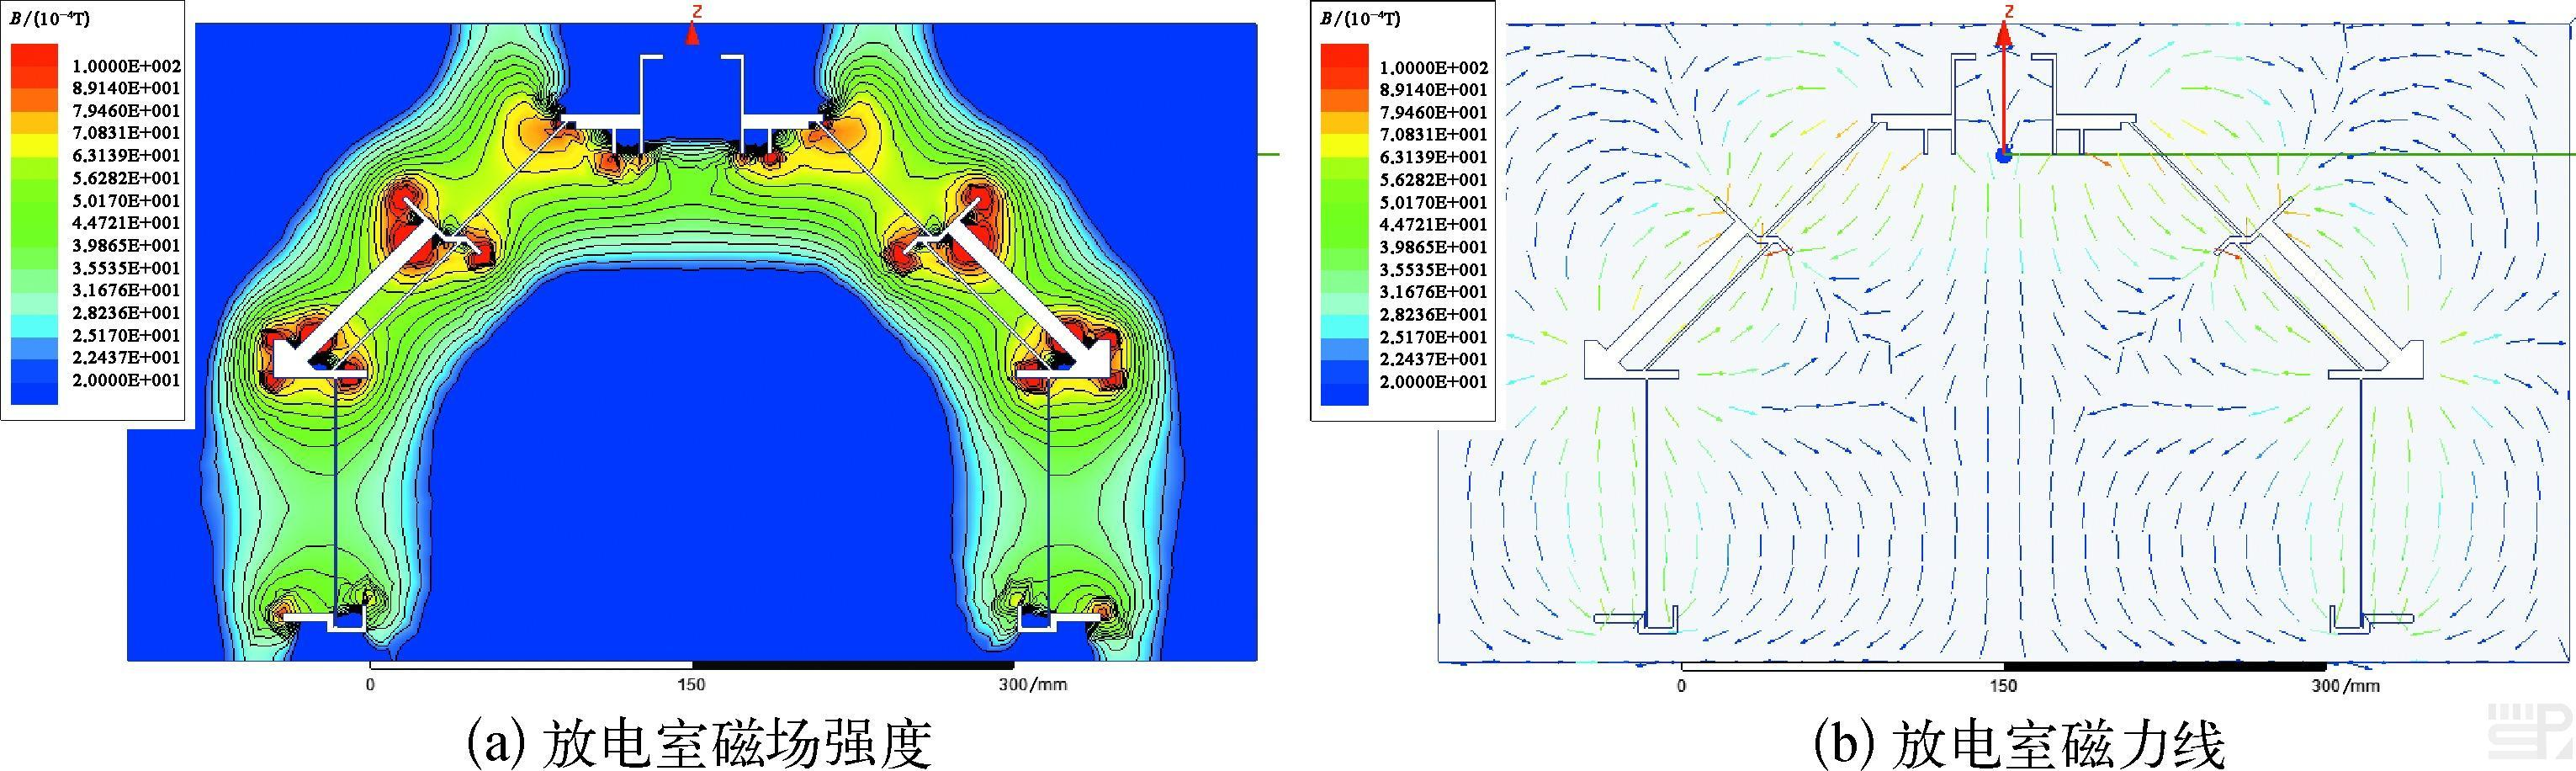
\includegraphics[width=0.9\textwidth]{imgs/柱形会切场理想磁场.png}
      \caption{柱形会切磁场磁力线示意图}
      \label{fig:cylindrical_cusp_magnetic_field_lines}
    \end{figure}

    \textbf{磁极数设计}核心诉求是在最少的磁极数下实现最佳的磁场构型，一般30cm一下的推力器使用三极场，30cm以上的推力器使用四极场。\textbf{最佳的磁极间距}设计取11-16cm，\textbf{阴极磁环半径}设计一般取3-4cm。

  \subsection{栅极组件设计}

  设计要求
  \begin{enumerate}
    \item 较高的束流密度需要更小的屏栅厚度和栅极间距，从而减小栅极孔直径增加孔数。
    \item 两栅间靠近程度受限于推力器口径，考虑温度导致形变带来的潜在短路风险，栅极间距不能过小。
    \item 屏蔽栅需要保证离子引出时不会直接轰击加速栅导致溅射腐蚀
    \item 加速栅厚度对于离子引出性能影响不大，因此往往加速栅厚度大于屏蔽栅厚度。
  \end{enumerate}

  \textbf{设计参数的经验公式}：

  屏孔孔径$d_s$与厚度$t_s$首先决定离子光学特性，其中$d_s$为其他参数设计过程的参考尺寸。

  \begin{figure}[htbp]
    \centering
    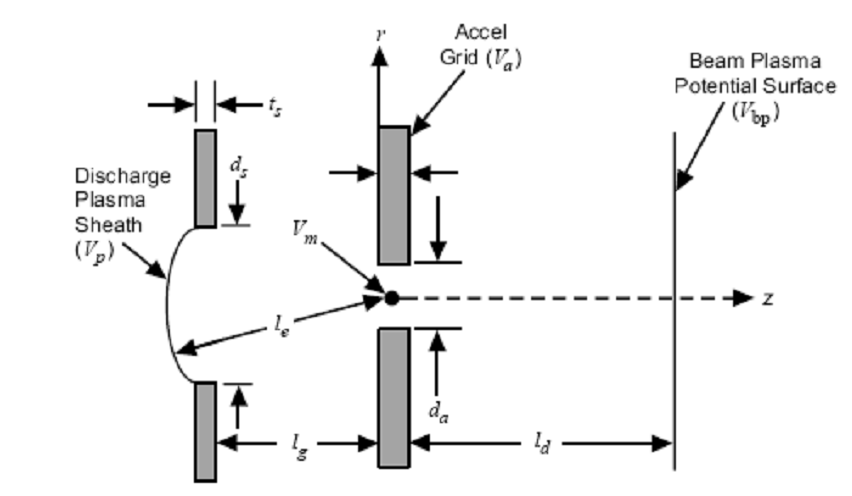
\includegraphics[width=0.5\textwidth]{imgs/栅孔尺寸系数.png}
    \caption{栅极组件几何参数示意图}
    \label{fig:grid_component_geometry}
  \end{figure}

  \begin{table}[htbp]
    \centering
    \caption{栅极组件设计参数经验公式}
    \label{tab:grid_design_parameters}
    \renewcommand{\arraystretch}{1.2}
    \begin{tabular}{lcc}
      \toprule
      参数 & 比值关系 & 取值范围 \\
      \midrule
      屏栅厚度 & $t_s / d_s$ & $0.125 \sim 0.175$ \\
      加速栅厚度 & $t_a / d_s$ & $0.2 \sim 0.4$ \\
      加速栅孔径 & $d_a / d_s$ & $0.6 \sim 0.7$ \\
      减速栅厚度 & $t_d / d_s$ & $0.2 \sim 0.4$ \\
      减速栅孔径 & $d_d / d_s$ & $0.8 \sim 0.9$ \\
      \bottomrule
    \end{tabular}
  \end{table}

  \textbf{栅极组件设计补偿}：大口径离子光学系统会使用球面设计应对热膨胀，但是会显著增加束流发散角导致性能损失（有球面形状带来的损失与加工后的周线不对位两部分产生）。通过调正其中一个\textbf{栅孔的中心距}，产生补偿作用让每一个单孔的束流向推力器的轴向偏转，从而低效球面形状带来的发散作用。

  \begin{figure}[htbp]
    \centering
    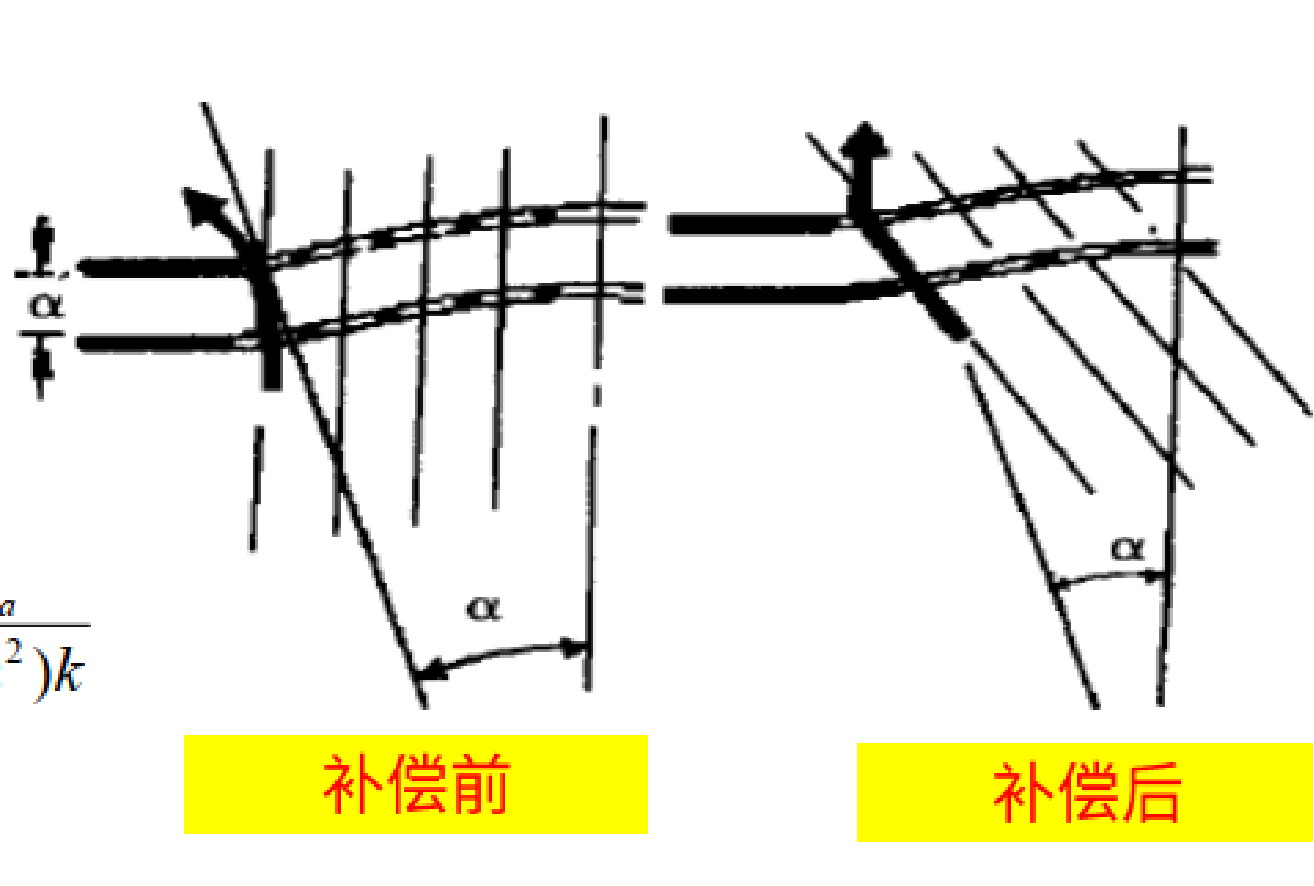
\includegraphics[width=0.5\textwidth]{imgs/光学系统补偿作用.png}
    \caption{栅孔补偿设计示意图}
    \label{fig:grid_hole_compensation_design}
  \end{figure}

  \textbf{束流引出性能设计}：
  归一化导流系数设计取最大归一化导流系数的$35\% \sim 50\%$,当栅极出现明显的离子截获时，所对应的K即为设计的使用上限：
  \begin{equation}
    K = \frac{I_b}{V_t^{3/2}} \left( \frac{l_e}{d_s}\right) ^2  \quad  l_e = \sqrt{(l_g + t_s)^2 + \frac{d_s^2}{4}} \quad K_{max} = \frac{I_b}{V_t^{3/2}} \left( \frac{l_e}{d_s}\right) ^2
  \end{equation}

  静总加速电压比R最佳取值为$0.75 \sim 0.90 $。

  栅极间距$l_g / d_s$：要求束流发散角小，同时抽取较大束流，最佳值取 $0.75 \sim 1.0$。

  \textbf{栅极塑件绝缘与支撑结构}：保证两栅极之阿金安全距离、保证栅极片之间连接固定的绝缘设计（方式放电室或外侧的等离子体或中性气体进入栅极之间的连接支撑区域）。

  \textbf{材料选择}：常用材料有钼、钛、碳基材料。主流材料依旧是使用钼，但是碳基材料拥有优异的热稳定性与耐溅射能力，可以解决栅极热变形与监视侵蚀的问题，但是力学强度低且制造工艺复杂。

  栅极安装环材料

  \textbf{栅极抗力学设计}间隙过小会有利于提高引出性能，但是产生更高的短路风险；对于球面栅极，拱高于弦的比值一般取0.5$\sim$0.6。

  \subsection{推力器耦合匹配设计}

  \textit{FUCK OFF. 这都什么乱七八糟的工程经验啊，记不住，完全记不住}
